\section{K-mer Abundance Histogram}
\label{sec:histogram}
To obtain information from reads, the reads are at first processed into $k$-mers. 
A $k$-mer is a substring of length exactly $k$. Using a read of length $r$ we produce 
$r-k+1$ $k$-mers. The same $k$-mer may be produced by multiple reads. If a $k$-mer occurs $i$ times
among all $k$-mers, we say its abundance is $i$. 

\begin{definition}
The $k$-mer abundance histogram is a sequence $f = f_1, f_2, f_3, \dots f_m$, 
where $f_i$ is the number of $k$-mers that occur in the input set exactly $i$ times 
and $m$ is the maximum observed abundance.
\end{definition}

Apart from estimating the genome size, several other methods in bioinformatics are also 
based on $k$-mers. For example, during genome assembly, the overlaps of $k$-mers are usually
considered instead of overlaps of reads. As the $k$-mer abundance histogram can be calculated
quickly, it can be also used for selection of an optimal $k$ in such methods \cite{Chikhi2013}.

Also note that the $k$-mer abundance histogram and many algorithms used for its computation
can be generalized to a histogram of any input items. Thus the applicability of this topic
outreaches the field of bioinformatics. 

\medskip

The value of $k$ must be set high enough to reduce the chance of two unrelated genome locations from 
producing the same $k$-mers\footnote{Under the assumption that each of \texttt{A, C, G, T}
nucleotide occurs at each position with probability $1/4$, we can expect approximately
$L^2 \cdot 4^{-k}$ \textit{collisions} in a genome of size $L$.}. However, with higher values of $k$,
each sequencing error affects more $k$-mers, thus increasing the fraction of erroneous $k$-mers
which produce problems in the downstream analysis. In our thesis we always use
the value $k=21$ as suggested in \cite{Williams2013, Hozza2015}.

\section{Computing K-mer Abundance Histogram}
\label{sec:algorithms}

A simple approach to compute $k$-mer abundance histogram would be firstly to compute $k$-mer
abundances -- the exact number of occurrences of each $k$-mer -- and then count different $k$-mers
with $j$ occurrences for each $j$. Since the role of $k$-mer abundances is important in
bioinformatics, there exist many tools that compute them. 
In the next subsection (\ref{sec:exact-algorithms}) we briefly summarize these algorithms.

However, counting $k$-mer abundances is a computationally demanding task for large inputs.
As we are only interested in the histogram, the problem of $k$-mer counting can be avoided,
allowing us to estimate the histogram very efficiently without an intermediate step.

\subsection{Exact K-mer Abundance Counting}
\label{sec:exact-algorithms}
In a naive hashing algorithm, a hash function $h$ would uniformly distribute strings of
length $k$ to a hash table $T$. We would store the number of occurrences of a $k$-mer
$s$ in the counter $T[h(s)]$. In a single scan through all the reads we
would then increment the appropriate counters. This solution works well for
millions of $k$-mers, but as the number of distinct $k$-mers increases,
we must use larger hash tables in order to prevent collisions.
This solution becomes much slower when the hash table $T$ becomes larger than RAM available.

A few techniques were used to decrease the time and memory consumption by a constant factor. 
These improvements allowed the hashing approach to be used in practice:

\begin{itemize}
\item Based on an observation that most of the $k$-mers with only one occurrence come from
erroneous reads, BFCounter \cite{Melsted2011} uses a Bloom filter to exclude rare $k$-mers
from hash table thus saving memory.

\item Jellyfish \cite{Marcais2011} software uses a thread-safe hash table utilizing the 
advantage of parallel computing.

\item To decrease the size of hash table, Disk Streaming of K-mers (DSK) \cite{Rizk2013}
algorithm scans the input data in more iterations, processing only a subset of $k$-mers
in each iteration. A second hash function is used to determine the subset (and the iteration) 
for each $k$-mer (a similar principle is used to randomly sample $k$-mers 
in section \ref{sec:simple-sampling}).
\end{itemize}

A different, but still memory-demanding, approach based on suffix arrays was
used in Tallymer software \cite{Kurtz2008}. A suffix array is a data structure
holding all suffixes of a string sorted in a lexicographical order. Suffixes with identical
prefixes of length at least $k$ represent different occurrences of a $k$-mer. Since
they are stored in a sorted order, abundances of $k$-mers can be computed by
grouping adjacent suffixes. 

\subsection{Approximating the Histogram}
As we drop the requirement to compute the exact histogram, it is no longer necessary to
store the abundance of each $k$-mer. This provides a way to reduce the amount of required
memory from dozens of gigabytes to hundreds of megabytes, allowing these computations to
be performed on a personal computer rather than on a cluster.  

To use all data available we must, however, still analyse every $k$-mer of every read so the
time complexity of the following algorithms will still be at least
linear in the number of $k$-mers.

\subsubsection{Simple sampling from $k$-mers}
\label{sec:simple-sampling}
The simplest optimization, which was used in a tool KmerGenie \cite{Chikhi2013},
is to sample from $k$-mers. With the parameter $s$, we can choose a hash function 
$\rho_s: \{A,C,G,T\}^k \rightarrow \{0, 1, \dots, s-1\}$ that uniformly distributes
the $k$-mers to $s$ buckets. Afterwards, we can compute the histogram by a naive
hashing approach or by any other algorithm presented in the previous section
\ref{sec:exact-algorithms} using only the $k$-mers that hashed to 0. 
Of all the distinct $k$-mers, only a randomly selected fraction of $1/s$ is considered.

The authors used value $s=1000$ in their experiments. As it can be seen from the
experimental data (fig. \ref{img:kmergenie-sampling-accuracy}), the approximation closely
follows the exact histogram $f$ at abundances with higher values of $f_i$ -- if enough
of unique $k$-mers of abundance $i$ were sampled. Fewer $k$-mers reach higher abundances
$i$ and thus even fewer of them are sampled, which leads to decreased relative precision
of approximation of lower values $f_i$. The authors did not include 
any analytical bounds of errors, however.

\begin{figure}
\centerline{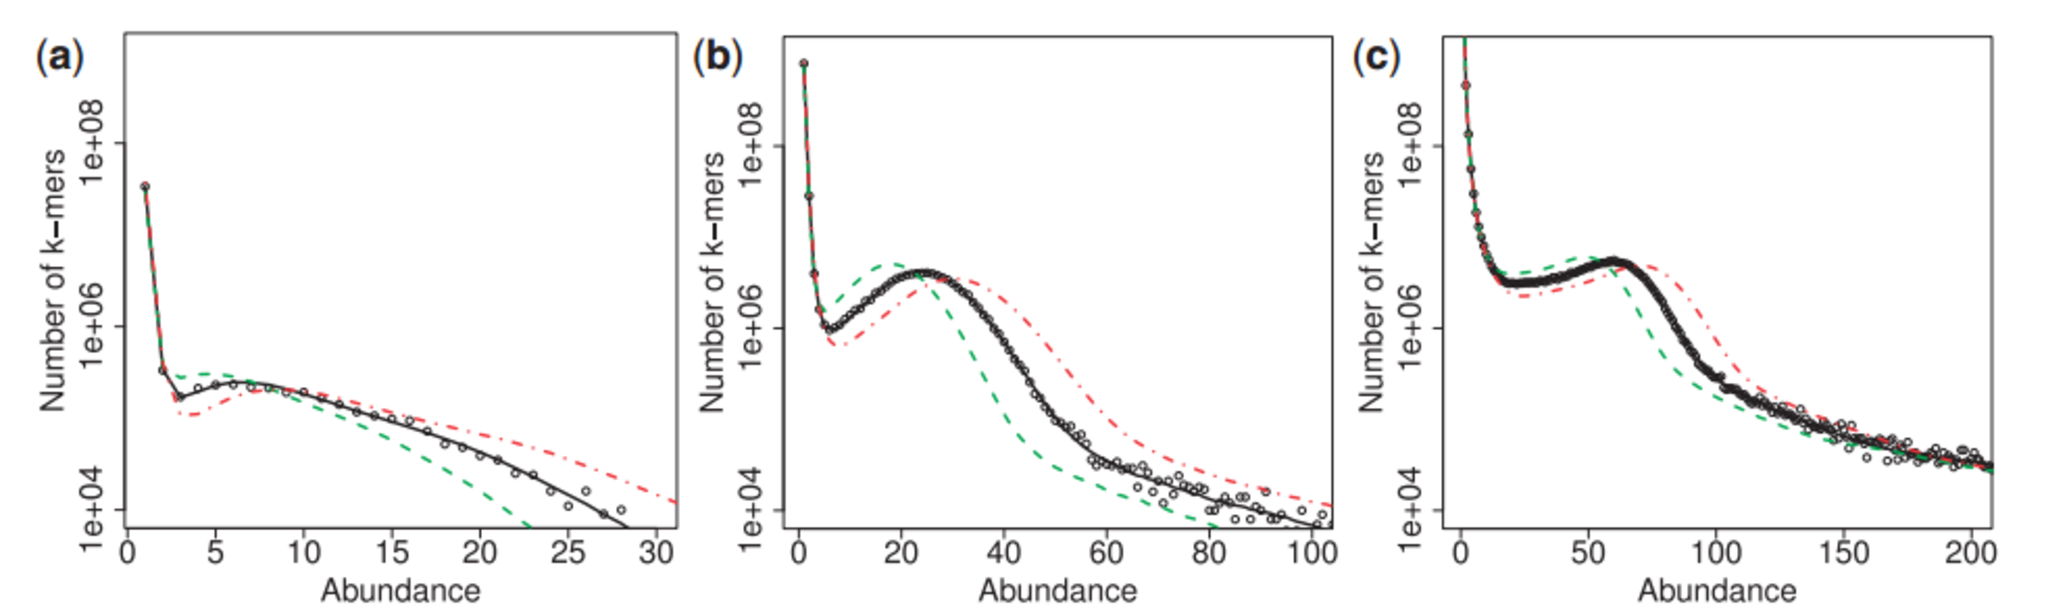
\includegraphics[width=1.1\textwidth]{images/kmergenie-sampling-accuracy.pdf}}
\caption[Accuracy of KmerGenie Sampling]{The accuracy of the sampling method. 
Reprinted from the original paper \cite{Chikhi2013}. 
The panels reflect three datasets. Each plot shows the exact
histogram curves for $k=51$ (solid black curve), $k=41$ (dash-dot red curve) 
and $k=61$ (dashed green curve). The approximate (sampled) histogram is
shown using black dots. Note that $f_i$ is shown on a log-scale, 
exaggerating the differences at lower $f_i$ values.}
\label{img:kmergenie-sampling-accuracy}
\end{figure}

\subsubsection{Multilevel sampling}
The inspiration for the next approach comes from a class of streaming algorithms.
Streaming algorithms are used to process a sequence of items (in our context $k$-mers) usually 
in only one pass with limited memory and time usage per item. A common problem solved by
streaming algorithms is counting distinct elements in a stream \cite{WikiStreamingAlg}.

These algorithms maintain an approximate summary or a sketch of the previously viewed
$k$-mers and with each new $k$-mer the sketch is updated. When all the $k$-mers are processed,
the sketch can be analyzed to provide the estimate of the $k$-mer abundance histogram.

\medskip

A streaming Algorithm 2 presented by Bar-Yossef et al. in 2002 \cite{Bar-Yossef2002} was
able to estimate the number of distinct elements in a stream ($F_0 = \sum_{i=1}^{m} f_i$)
with theoretical guarantees. 

In 2014 Melsted and Halldórsson \cite{Melsted2014} implemented this algorithm and used it for
$k$-mer counting. Their algorithm KmerStream also extended Algorithm 2, since it was able
to estimate the number of $k$-mers with abundance one, $f_1$. According to authors, this
algorithm is at least three times faster than KmerGenie and it can use ten times less memory.

KmerStream was further improved by Sivadasan et al.\ in 2016 \cite{Sivadasan2016}
and their software Kmerlight was able to estimate the whole histogram ($f_1, f_2, \dots , f_m$).
The authors also included theoretical bounds of approximation errors.

As we focus greatly on Kmerlight in our work, we will describe Kmerlight in detail 
in the next chapter (\ref{sec:kmerlight}).
